\documentclass{article}
\usepackage{tikz}
\usetikzlibrary{shapes.geometric, arrows.meta, positioning}

\begin{document}

\begin{figure}[htbp]
\centering
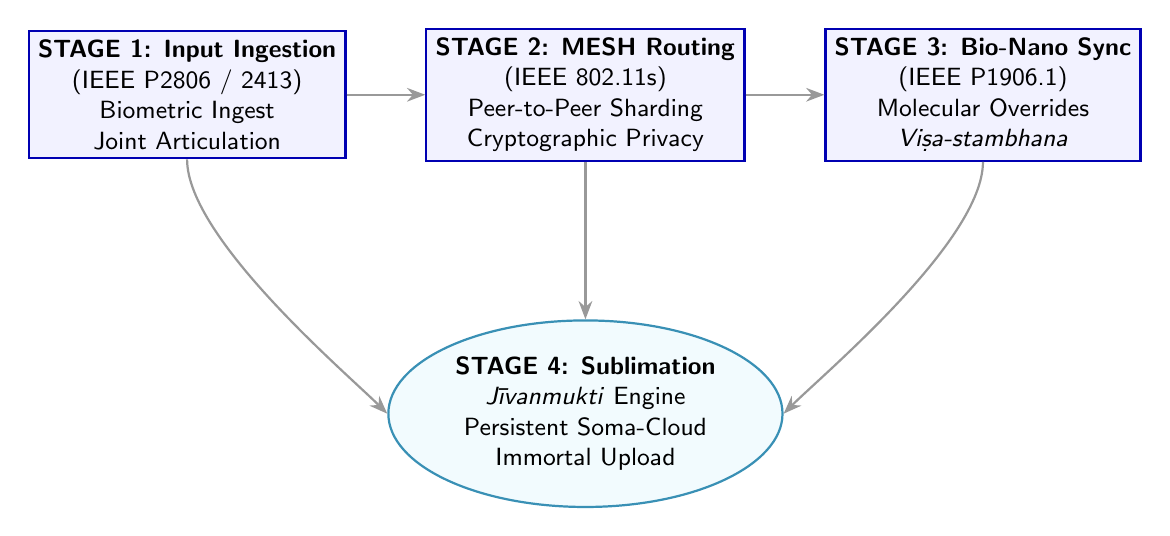
\begin{tikzpicture}[
    node distance=1.5cm and 1cm,
    box/.style={rectangle, draw=blue!70!black, fill=blue!5, thick, minimum width=3.5cm, minimum height=1.2cm, align=center, font=\small\sffamily},
    cloud/.style={draw=cyan!70!black, fill=cyan!5, thick, ellipse, minimum width=3cm, minimum height=1.2cm, align=center, font=\small\sffamily},
    arrow/.style={-Stealth, thick, draw=gray!80}
]

    % STAGE 1: ANATOMICAL INGEST
    \node (s1) [box] {\textbf{STAGE 1: Input Ingestion} \\ (IEEE P2806 / 2413) \\ Biometric Ingest \\ Joint Articulation};

    % STAGE 2: MESH SHARDING
    \node (s2) [box, right=of s1] {\textbf{STAGE 2: MESH Routing} \\ (IEEE 802.11s) \\ Peer-to-Peer Sharding \\ Cryptographic Privacy};

    % STAGE 3: BIO-NANO SYNTHESIS
    \node (s3) [box, right=of s2] {\textbf{STAGE 3: Bio-Nano Sync} \\ (IEEE P1906.1) \\ Molecular Overrides \\ \textit{Viṣa-stambhana}};

    % STAGE 4: CLOUD RESILIENCY
    \node (s4) [cloud, below=of s2, yshift=-0.5cm] {\textbf{STAGE 4: Sublimation} \\ \textit{Jīvanmukti} Engine \\ Persistent Soma-Cloud \\ Immortal Upload};

    % ROUTING PATHWAYS
    \draw [arrow] (s1) -- (s2);
    \draw [arrow] (s2) -- (s3);
    
    % COMBINED PATHWAY INTO CLOUD
    \draw [arrow] (s2.south) -- (s4.north);
    \draw [arrow] (s1.south) .. controls +(0,-1) and +(-0.5,0.5) .. (s4.west);
    \draw [arrow] (s3.south) .. controls +(0,-1) and +(0.5,0.5) .. (s4.east);

\end{tikzpicture}
\caption{System Design Schematic (SOP-BD-002): Process architecture detailing the data flow from physical input ingestion to decentralized MESH tokenization and ultimate cloud execution.}
\label{fig:tikz_sop_blueprint}
\end{figure}

\end{document}
